\RequirePackage{luatex85} %https://tex.stackexchange.com/a/315027/152544
\documentclass[tikz, border=10pt]{standalone}

\usepackage[compat=1.1.0]{tikz-feynman}

% c.f. https://tex.stackexchange.com/a/298288/152544
\tikzset{
 pics/fatjet/.style args={#1}{
  % default rotation: 0 degrees (jet progressing to right)
  code={
   \draw [fill=#1!30, thick,join=round](0, 0) -- (4, -1) -- (4, 1) --cycle;
   \draw [fill=#1!30, thick](4, 0) ellipse (.25 and 1);
  }
 }
}

\begin{document}

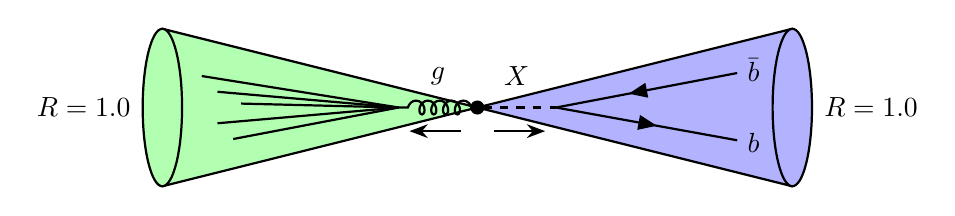
\begin{tikzpicture}[thick]
 \path (0, 0)  pic {fatjet=blue};
 \path (0, 0)  pic [rotate=-180] {fatjet=green};

 \begin{feynman}
  \vertex [dot] (origin) {};
  \vertex [right=1cm of origin, label={[xshift=-0.5cm, yshift=0.15cm]\(X\)}] (X);
  \vertex [above right=0.20cm and 2.3cm of X] (b1) {\(\bar{b}\)};
  \vertex [below right=0.20cm and 2.3cm of X] (b2) {\(b\)};
  \vertex [left=1cm of origin, label={[xshift=0.5cm, yshift=0.15cm]\(g\)}] (jet);
  \vertex [above left=0.20cm and 2.3cm of jet] (q1);
  \vertex [below left=0.20cm and 2.3cm of jet] (q2);
  \vertex [above left=0.40cm and 2.5cm of jet] (q3);
  \vertex [below left=0.40cm and 2.1cm of jet] (q4);
  \vertex [above left=0.05cm and 2.0cm of jet] (q5);
  \vertex [right=5cm of origin] (largeR_signal) {$R = 1.0$};
  \vertex [left=5cm of origin] (largeR_jet) {$R = 1.0$};
  \diagram* {
  (origin) -- [scalar, momentum'={}, style={pos=0.2}] (X) -- [anti fermion] (b1),
  (X) -- [fermion] (b2),
  (origin) -- [gluon, momentum={}] (jet),
  (jet) -- (q1),
  (jet) -- (q2),
  (jet) -- (q3),
  (jet) -- (q4),
  (jet) -- (q5),
  };
 \end{feynman}
\end{tikzpicture}
\end{document}
